In particular, the following factors were tested: an object's composition, geometry (thickness), and position in the X-ray detector. To test any of these factors, one must first determine how to obtain the effective energy, $E_{\text{eff}}$, from an X-ray image. The initial X-ray intensity the moment before encountering the object, $I_0$, and resulting intensity upon exit, $I$, are related by the exponential attenuation law:

\begin{equation}
    I = I_0e^{-\mu x},
\label{eq:AttnLaw}
\end{equation}

where $\mu$ is the attenuation coefficient of the material and $x$ is the distance the X-ray travels through the material.

Solving Eq (\ref{eq:AttnLaw}) for $\mu$ yields the following relationship:

\begin{equation}
    \mu = \frac{\ln{(I_0/I)}}{x}.
\label{eq:mu}
\end{equation}

With $\mu$ being a function of effective energy, one can refer to experimental data to relate a value of $\mu$ to its associated effective energy. Therefore, with NIST's Tables of X-Ray Mass Coeffecients \cite{NIST} and Eq (\ref{eq:mu}), one can find the $I_0$, $I$, and $x$ for a particular x-ray image and determine the effective energy of the spectrum at the set kVp.

To obtain these values, a small surgical X-ray machine called the GE MiniView 6800 Mini C-Arm was used in the anatomy lab at Saint Vincent College, as described in figure 1. In order to test the composition dependence of the effective energy, images were taken of aluminum, iron, magnesium, water, and a plastic scintillator. Several images were taken for each object, with kVps ranging from 40 keV to 60 keV. For each image, the object was placed in the center of the imaging area of the C-Arm, and the kVp was set with the kVp controller located on the machine. Once ready, a remote was used to activate the machine, which then sent X-rays from the tube toward the imaging area.

\begin{figure}[H]
    \centering
	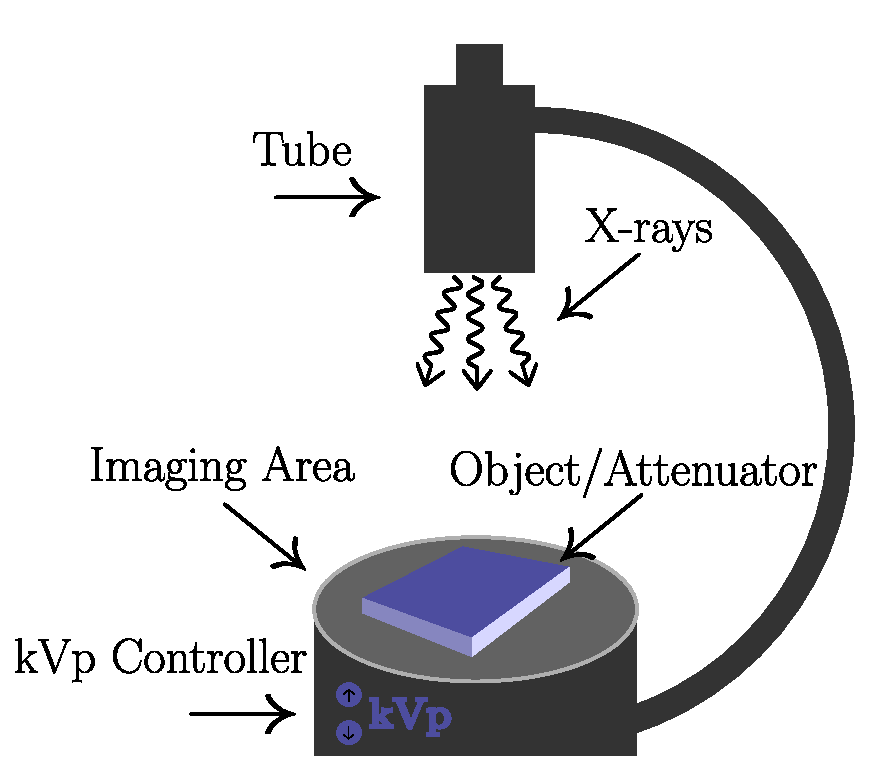
\includegraphics[scale=0.7]{CArmDiagram.pdf}
	\label{figure:CArmDiagram}
	\caption{}
\end{figure}

To test the geometrical dependence on effective energy, an image was taken of a slightly thinner sheet of aluminum and compared to an image of the thicker aluminum used for the composition experiment. Additionally, for the position dependence, an image was taken of aluminum shifted towards the edge of the imaging area. For both of these experiments, the images taken were compared to images taken at the same kVp to observe only the change in effective energy due to the factors adjusted, rather than a change due to a shift in the spectrum.

With images taken, $I/I_0$ had to be extracted from each image to determine $\mu$ using Eq (\ref{eq:mu}). With $I/I_0$ acting as the intensity relative to initial intensity, one can think of this ratio as the probability of x-ray transmission. In particular, if we have $N$ photons passing through an object, $I/I_0$ describes what percentage of particles will pass through (e.g if equal to 1, all have passed, and if 0, all were attenuated). Similarly, if we imagine a single photon passing through an object, $I/I_0$ will give the probability of that photon passing through the object. Therefore, if a photon passes through N objects, 

\begin{equation}
    \frac{I_N}{I_0} = \prod_{j=1}^{N} \frac{I_j}{I_0},
   \label{eq:ProbI}
\end{equation}

where $I_j$ is the intensity of a ray as it exits the $j$-th object and $I_N$ is the intensity of a ray as it exits the $N$-th object.

Consider the X-ray image in figure 2; along an X-ray's journey from the tube to the detector, it encounters two different attenuators, the air and the object we place in the imaging area (with the machine setting a completely non-attentuated beam equal to 1 in the image, where 1 is white and 0 is black, the only values we can measure from pixel inspection are the relative intensities of the x-ray. Because of this, $I$ will now simply refer to the pixel intensity (0-1) and will replace $I/I_0$). In the image, $I$ becomes $I_{\text{bkg}}$ and $I_{\text{ctr}}$ for the pixel intensity in the background and center of the image, respectively. $I_{\text{bkg}}$ refers to attenuation caused by the air, while $I_{\text{ctr}}$ refers to attenuation caused by both the air and the object. Using Eq (\ref{eq:ProbI}), one can show that $I_{\text{ctr}} = I_{\text{bkg}} I_{\text{obj}}$, where $I_{\text{obj}}$ is the attenuation caused by the object. Therefore, the attenuation caused by the object, and the pixel intensity if there were no attenuation from the air is given by

\begin{equation}
    I_{\text{obj}} = \frac{I_{\text{ctr}}}{I_{\text{bkg}}}
\label{eq:IObj}
\end{equation}

\begin{figure}[H]
    \centering
	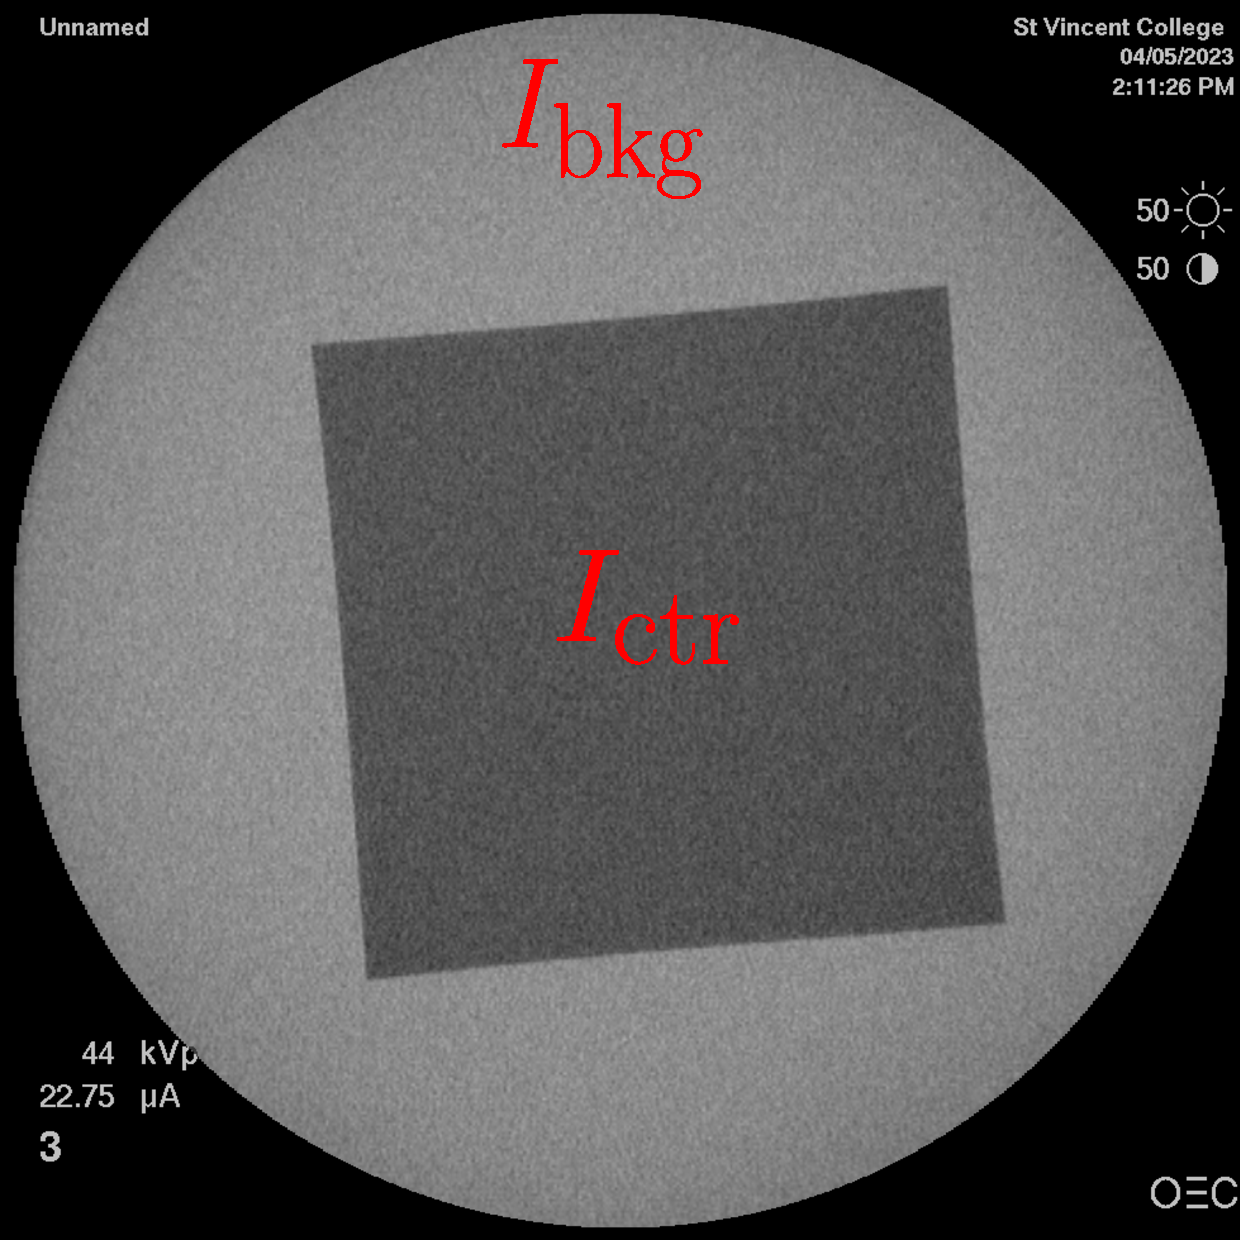
\includegraphics[scale=0.4]{IntensityDiagram.pdf}
	\label{figure:IntensityDiagram}
	\caption{}
\end{figure}

With this relative intensity and the thickness of object, the attenuation coefficient and effective energy of the interaction was determined using equation \ref{eq:AttnLaw}.